\documentclass[10pt,a4paper]{article}
\usepackage[margin=1.6cm]{geometry}
\usepackage[T1]{fontenc}
\usepackage[utf8]{inputenc}
\usepackage{lmodern}
\usepackage{booktabs}
\usepackage{graphicx}
\usepackage{xcolor}
\usepackage{hyperref}
\usepackage{enumitem}
\usepackage{amsmath}
\usepackage{amssymb}
\usepackage{titlesec}
\usepackage{fancyhdr}

\definecolor{navy}{HTML}{004E7C}
\definecolor{slate}{HTML}{4A5568}
\definecolor{accent}{HTML}{D55E00}

\hypersetup{colorlinks=true, linkcolor=navy, urlcolor=navy}
\titleformat{\section}{\large\bfseries\color{navy}}{}{0em}{}[\titlerule]
\titlespacing*{\section}{0pt}{8pt}{4pt}
\setlist[itemize]{noitemsep, topsep=2pt, leftmargin=1.4em}

\pagestyle{fancy}
\fancyhf{}
\lhead{\small\color{slate} Fundamentals of Machine Learning (UAB) --- Follow-up \#1 Progress Brief (Dec 4)}
\rhead{\small\color{slate} Project Team 05}
\cfoot{\small\thepage}

\begin{document}

\begin{center}
  {\LARGE\bfseries\color{navy} Follow-up \#1 Deliverable: Obtain, Scrub \& Explore}\\[4pt]
  {\large Predicting Formula 1 Points Finishes (2010--2024): Pre-Race Data Pipeline, Zero-Leakage Verification \& Exploratory Analysis}\\[5pt]
  {\small\color{slate} \textbf{Team 05:} Marc Font Hostalet, David Redrejo P\'erez, Elias Barreiro Pena \quad|\quad \textbf{Notebook:} \texttt{notebooks/01\_followup1\_obtain\_scrub\_explore.ipynb}}
\end{center}
\vspace{-4pt}

\section{1. Research Hypothesis \& Alignment with Instructor Guidance}
We frame Formula 1 points-finish prediction (\texttt{top10} $= \mathbb{I}[\text{positionOrder} \le 10]$) across the modern Top-10 scoring era (\textbf{2010--2024}, 305 Grands Prix, $n=6{,}436$, positive rate \textbf{47.39\%}) using \textbf{26 strictly pre-race features} partitioned into three disjoint factor groups: \textbf{Group A (Qualifying \& Grid, 8)}, \textbf{Group B (Rolling Constructor \& Driver Form, 11)}, and \textbf{Group C (Historical Circuit Characteristics, 7)}. We hypothesize that Groups A and B dominate predictive power over Group C, enabling regularized linear models (Logistic Regression, Linear SVM) to match or exceed non-linear ensembles while beating the scrubbed \texttt{grid} $\le 10$ heuristic baseline (\textbf{76.91\%}).

\begin{itemize}
  \item \textbf{Zero In-Race Leakage:} Excluded \texttt{lap\_times}, \texttt{pit\_stops}, target-race \texttt{status}, race time/laps, and post-race standings; enforced via automated schema assertions and adversarial mutation tests (\texttt{future\_mutation\_max\_abs\_diff = 0.0}, \texttt{same\_race\_mutation\_max\_abs\_diff = 0.0}).
  \item \textbf{Season-Based Temporal Split:} Development = \textbf{2010--2021} (12 seasons, $n=5{,}077$; 5-fold expanding-window CV on 2017--2021); Held-out Test = \textbf{2022--2024} Ground-Effect era (3 seasons, $n=1{,}359$). All exploratory feature-target analyses below are strictly restricted to 2010--2021.
  \item \textbf{Domain Scrubbing Wins:} (i) Re-mapping 85 \texttt{grid == 0} pit-lane starts to back-of-grid (\texttt{n\_entries + 1}) raises the \texttt{grid} $\le 10$ baseline by \textbf{+0.89 pp} ($76.03\% \rightarrow 76.91\%$); (ii) Canonicalizing 23 raw constructors into 13 continuous lineages resolves Ergast rebrand discontinuities (including Kick Sauber reverting to 2018 ID 15 in 2024); (iii) Race-level shifting prevents same-race teammate leakage.
\end{itemize}

\begin{figure}[h!]
  \centering
  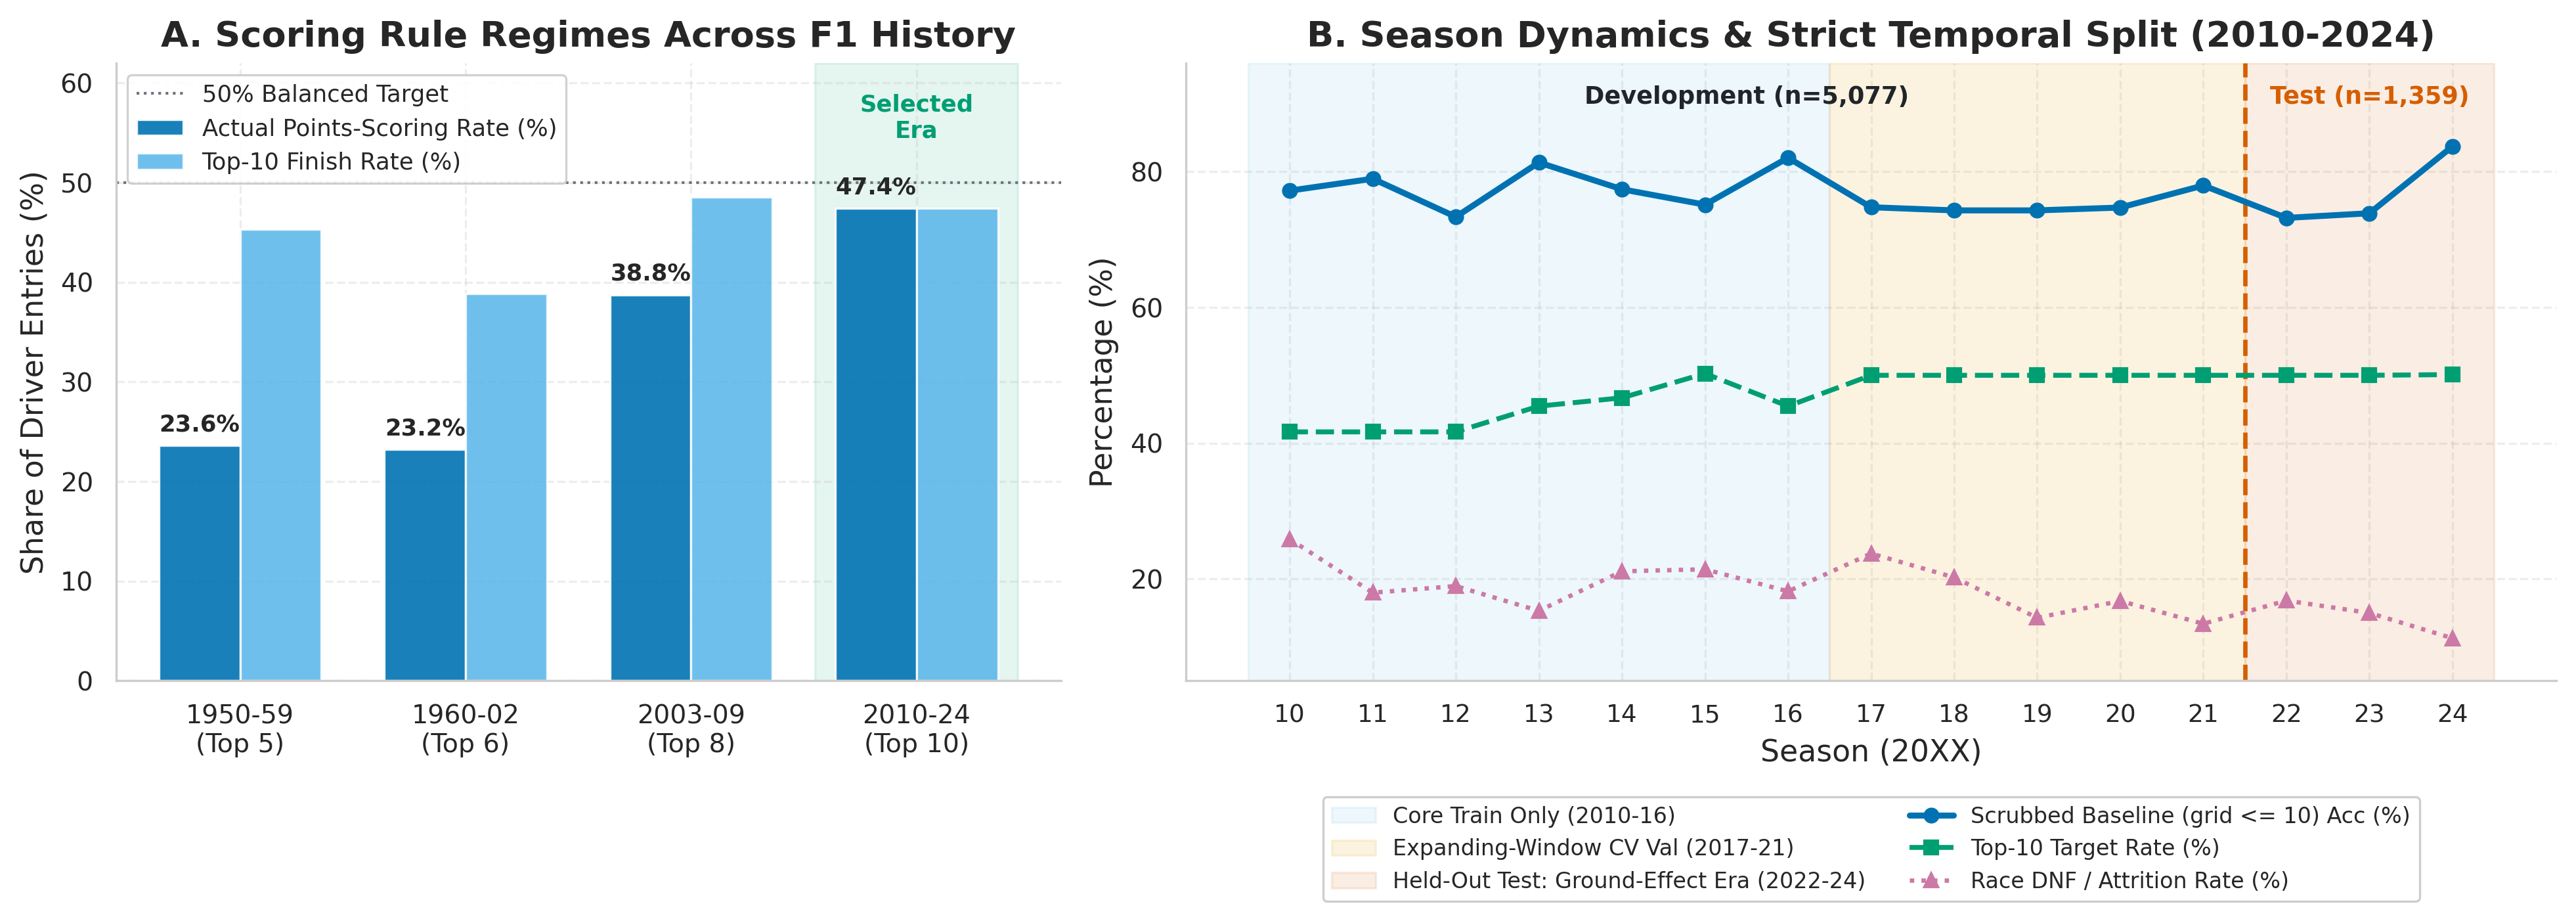
\includegraphics[width=0.98\textwidth]{../figures/followup1/fig01_scoring_eras_and_temporal_split.png}
  \vspace{-6pt}
  \caption{\small Historical FIA scoring rule shifts justifying restriction to 2010--2024 (left) and the strict season-based Development / Expanding-CV / Held-out Test protocol (right).}
\end{figure}

\begin{figure}[h!]
  \centering
  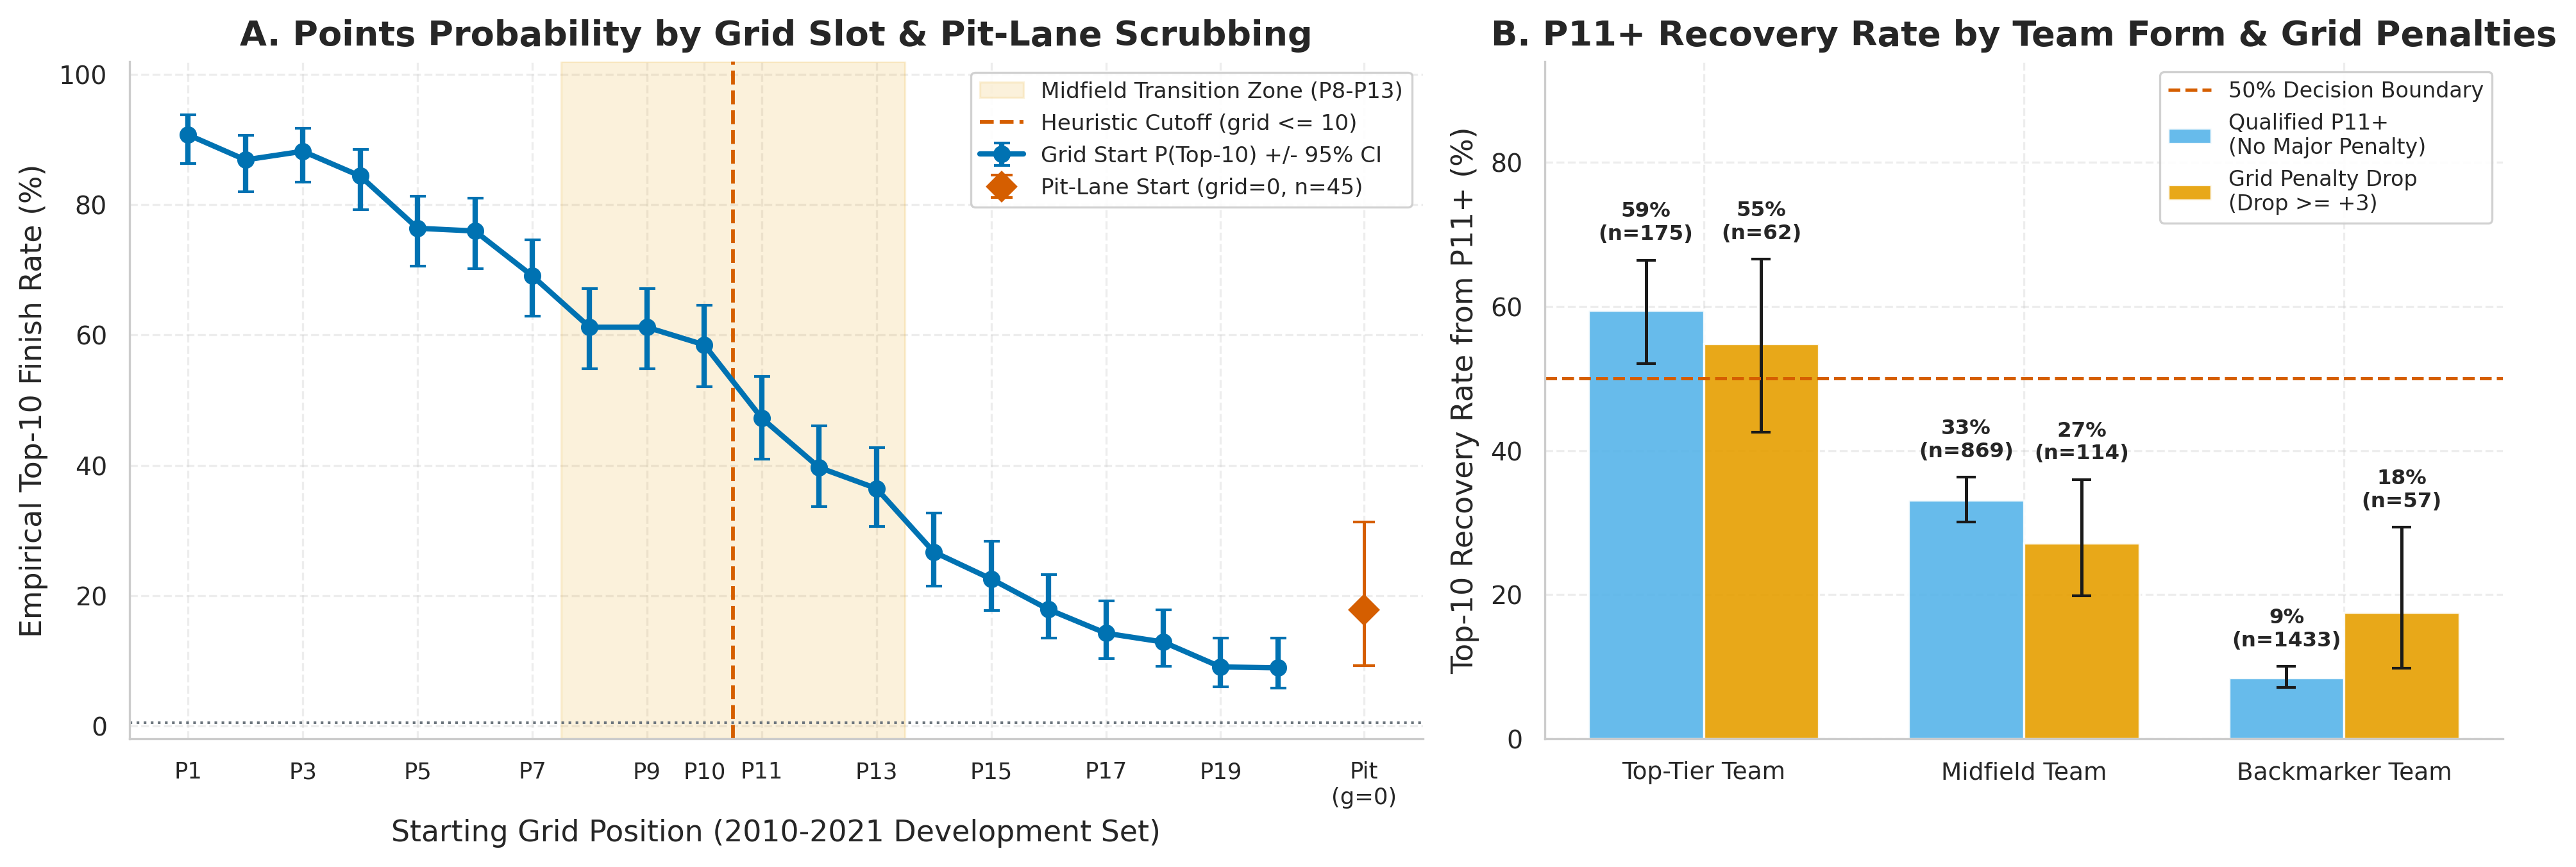
\includegraphics[width=0.98\textwidth]{../figures/followup1/fig02_grid_vs_top10_and_pitlane_scrub.png}
  \vspace{-6pt}
  \caption{\small Empirical $P(\text{Top-10} \mid \text{Grid})$ with 95\% Wilson CIs highlighting the P8--P13 midfield transition zone where \texttt{grid} $\le 10$ drops to 59.6\% (left), and P11+ recovery rates showing top teams score 55--59\% despite starting outside Top-10 (right).}
\end{figure}

\newpage

\section{2. Exploratory Signal Across the Three Factor Groups (Dev 2010--2021)}
\begin{table}[h!]
  \centering
  \footnotesize
  \setlength{\tabcolsep}{5pt}
  \begin{tabular}{lccccc}
    \toprule
    \textbf{Pre-Race Factor Group} & \textbf{\# Feat.} & \textbf{Mean AUC} & \textbf{Max AUC (Top Feature)} & \textbf{Mean MI} & \textbf{Max VIF} \\
    \midrule
    Group A: Qualifying \& Grid Context & 8 & 0.7088 & \textbf{0.8419} (\texttt{qualy\_pos}) & 0.1180 & 139.9 \\
    Group B: Rolling Constructor \& Driver Form & 11 & \textbf{0.7277} & 0.8346 (\texttt{const\_season\_pts}) & \textbf{0.1282} & 22.2 \\
    Group C: Historical Circuit Characteristics & 7 & 0.5765 & 0.7044 (\texttt{const\_circ\_top10}) & 0.0288 & 8.4 \\
    \bottomrule
  \end{tabular}
  \vspace{-4pt}
  \caption{\small Univariate discriminative power (nats for MI) and multicollinearity across the three disjoint pre-race factor groups on Development seasons (2010--2021, $n=5{,}077$).}
\end{table}

\begin{figure}[h!]
  \centering
  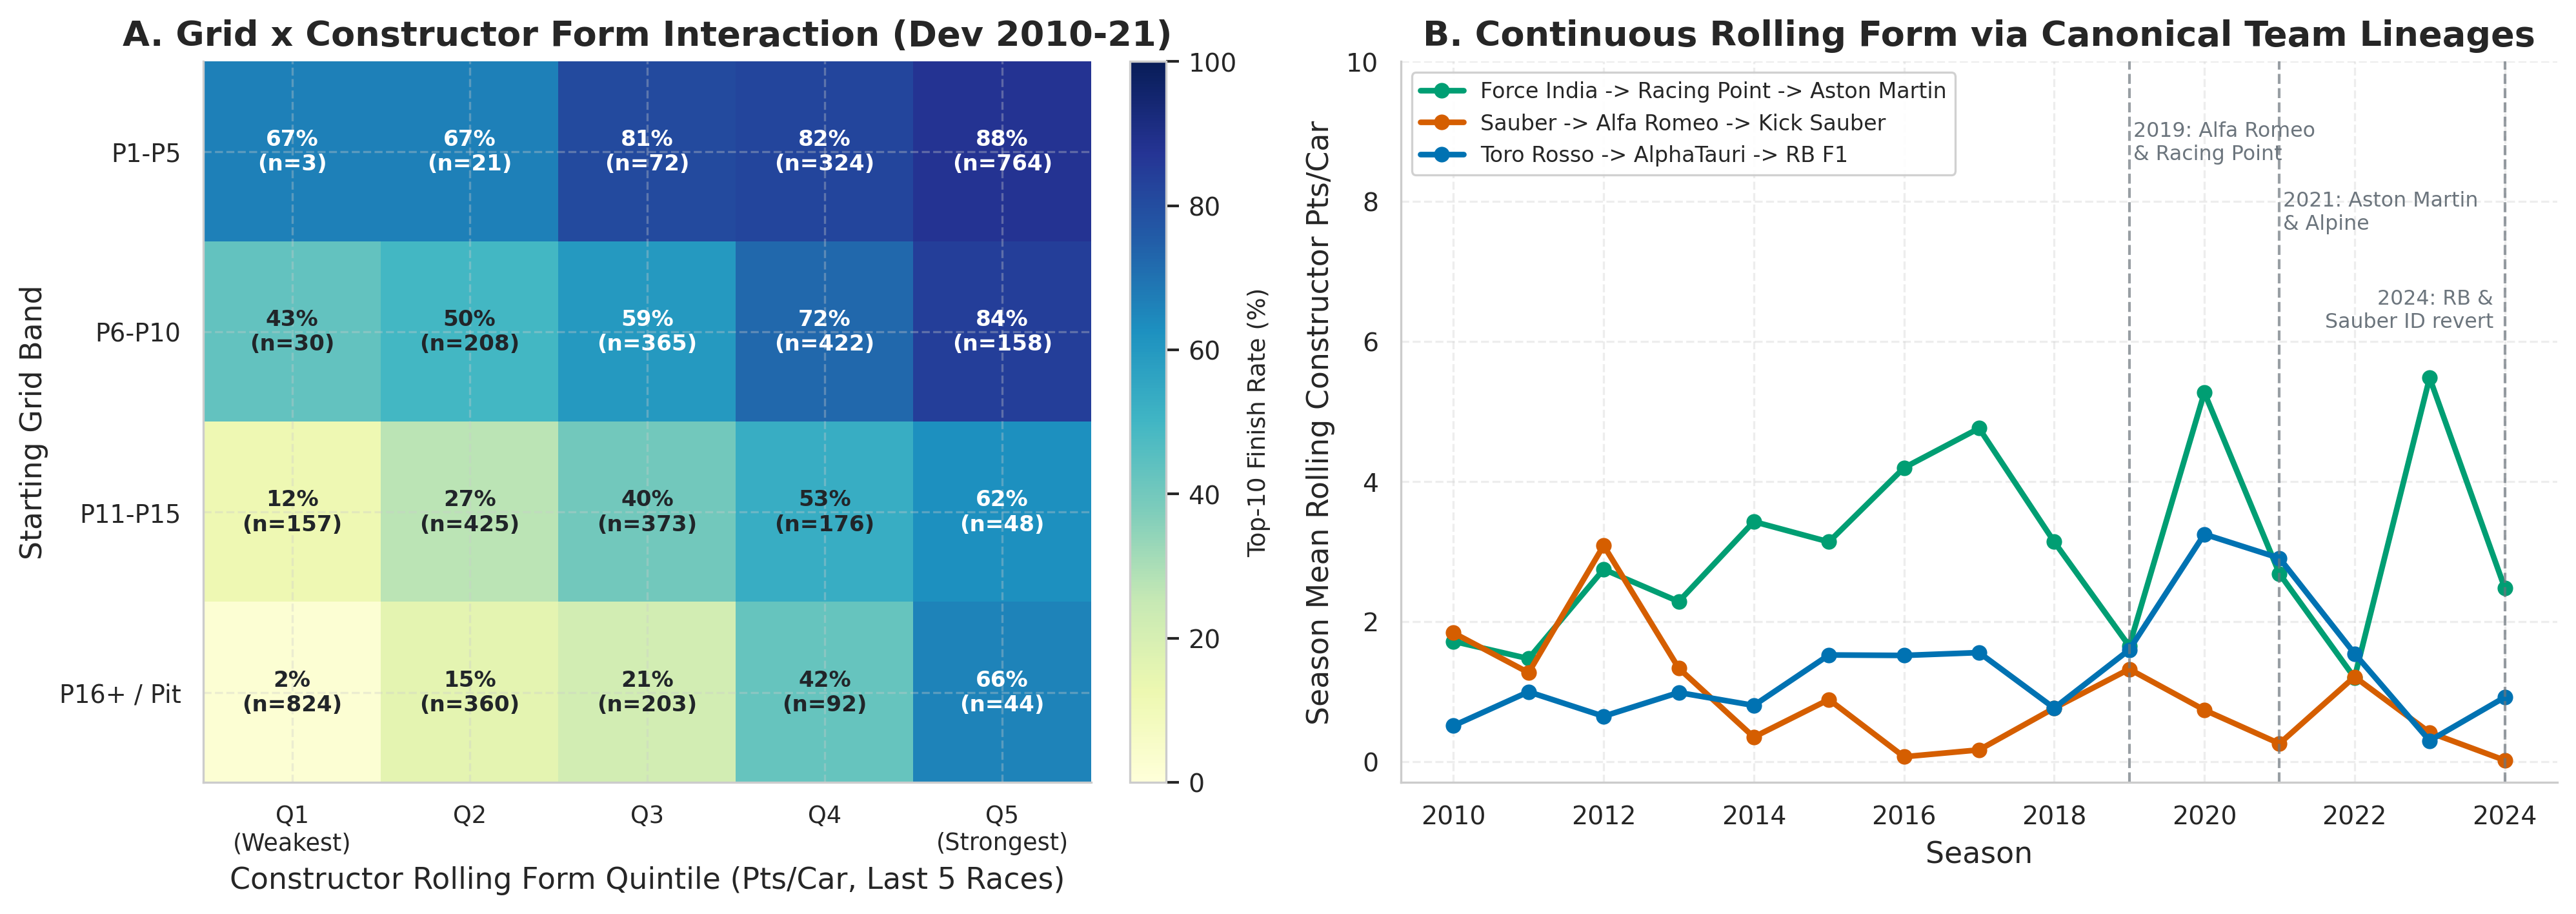
\includegraphics[width=0.98\textwidth]{../figures/followup1/fig04_constructor_momentum_and_lineage.png}
  \vspace{-6pt}
  \caption{\small Left: Grid band $\times$ Constructor rolling form quintile interaction showing P16+ starts score 66\% for Q5 teams vs 2\% for Q1 backmarkers, while P6--P10 starts drop to 43\% for Q1 teams. Right: Longitudinal continuity restored across team rebrands.}
\end{figure}

\begin{figure}[h!]
  \centering
  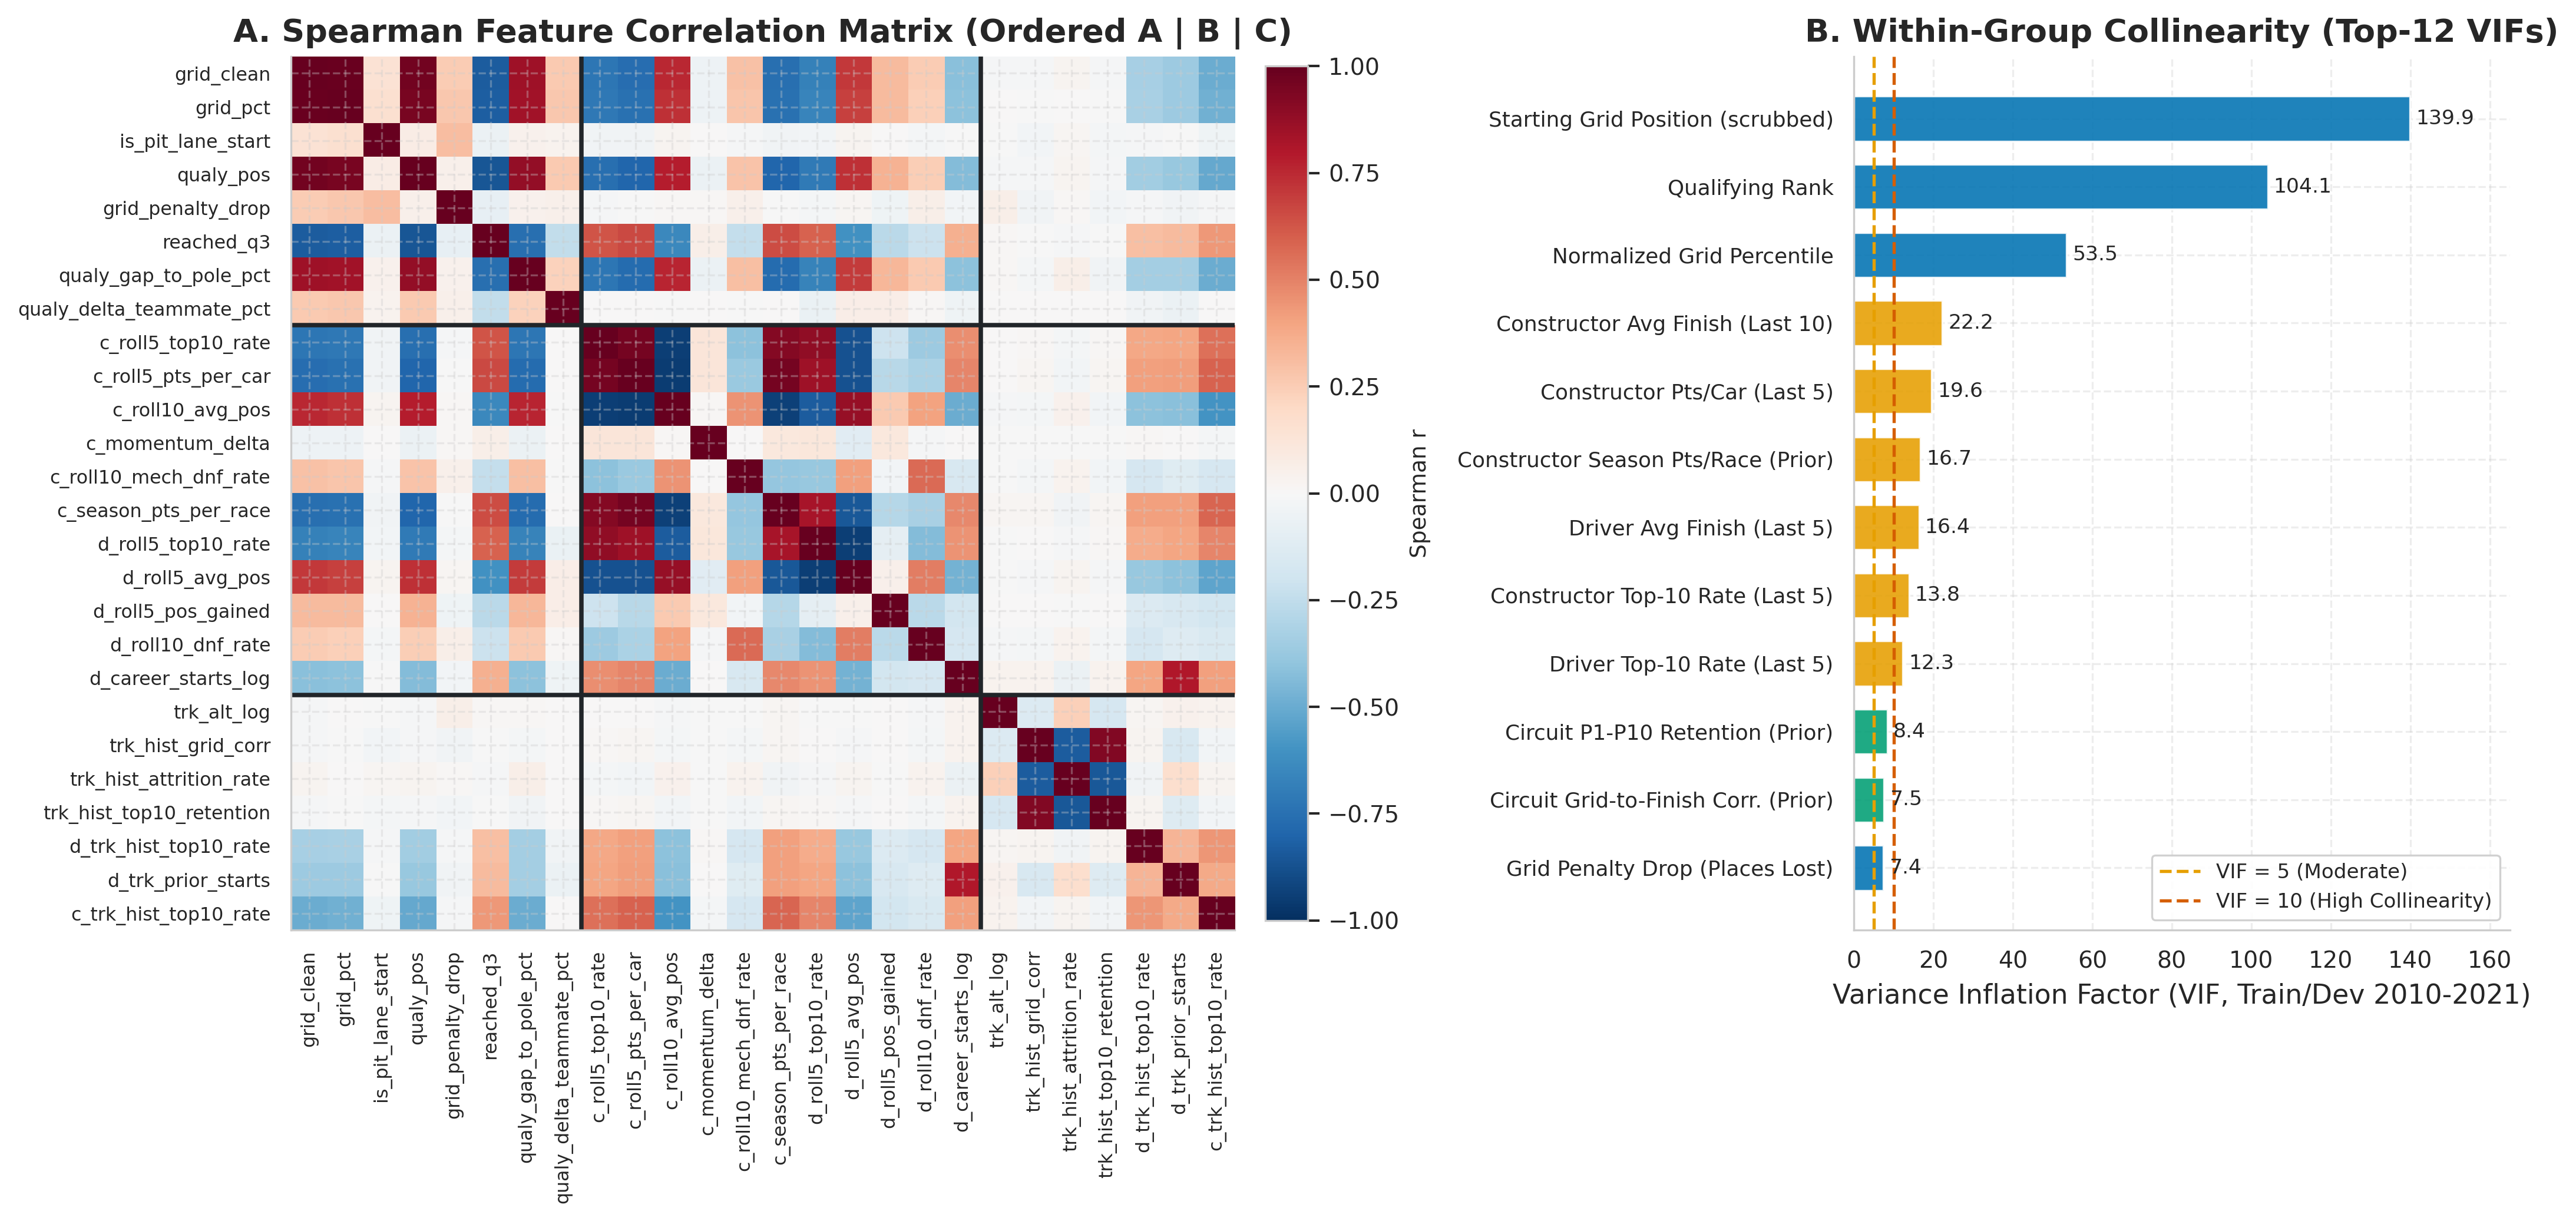
\includegraphics[width=0.98\textwidth]{../figures/followup1/fig06_correlation_matrix_and_multicollinearity.png}
  \vspace{-6pt}
  \caption{\small Group-ordered Spearman correlation heatmap (left) and Top-12 Variance Inflation Factors (right), establishing strong within-group collinearity that directly motivates L1/L2 regularization in Follow-up \#2.}
\end{figure}

\section{3. Readiness for Follow-up \#2 (Dec 11: Model \& iNterpret)}
The verified, leakage-free processed dataset (\texttt{data/processed/f1\_modeling\_2010\_2024.parquet}) is finalized. Follow-up \#2 will: (1) benchmark 9 course models (L2/L1 Logistic, Linear/RBF SVM, Gaussian NB, k-NN, Decision Tree, Random Forest, Gradient Boosting) against 3 baselines under expanding-window seasonal CV; (2) execute the complete $2^3 - 1 = 7$-subset ablation matrix with exact Shapley attributions ($\phi_A, \phi_B, \phi_C$); and (3) perform regularization sweeps, rolling-window sensitivity tests, and post-hoc irreducible DNF error decomposition on 2022--2024.

\end{document}
